\subsection{{\tt eaaCanal} package} \label{fceaacanal}

The {\tt eaaCanal} flood control assessor quantifies the volume of
excess in an EAA canal and reconciles the canal's flood control needs
with regional water supply requirements at each outlet structure. The
{\tt eaaCanal} flood control assessor routes excess flow to its outlet
structures in response to the following objectives (from highest to
lowest priority): (1) use excess flow to meet local and downstream
water supply demand; (2) store excess flow in reservoirs; (3) treat
excess flow in Stormwater Treatment Areas; and (4) release untreated
excess flow through the tailNode outlet structures.

A flowchart schematic representation of the eaaCanal flood control
{\tt Assess()} function is shown in Figure \ref{fig:eaaCanalFC}. 

\begin{figure}[!htb]
 \begin{center}
  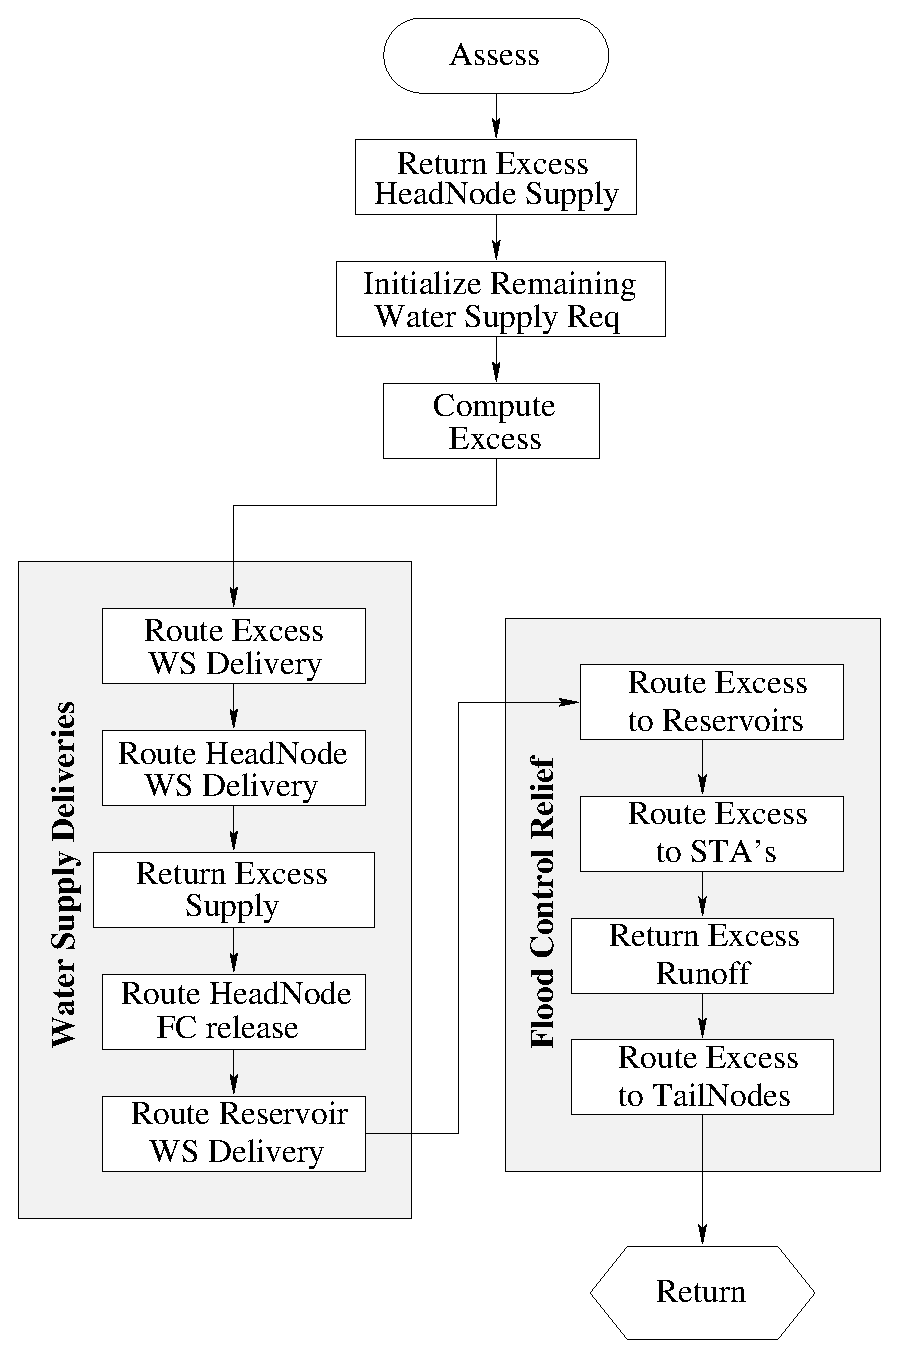
\includegraphics[scale=.5]{Graphics/eaaCanalFC}
  \caption{\label{fig:eaaCanalFC} EAA canal flood control Assess() function}
 \end{center}
\end{figure}

The {\tt eaaCanal} package uses the following procedures to address
the water supply and flood control needs for an EAA canal:

\begin{enumerate}

 \item Return excess headNode supply.  Excess water supply deliveries
   can occur when an EAA canal has multiple headNodes, and a water
   supply delivery from one headNode can be offset by a flood control
   release from another.  The excess supply is quantified and returned
   to the upstream source.

 \item Initialize remaining water supply requirement for each EAA
   canal outlet, using water supply requirements computed by the EAA
   canal's water supply assessor (see Section \ref{wseaacanal}).

 \item Compute EAA canal excess flow.  Excess volume is defined as the
   portion of projected EAA canal storage that exceeds the flood
   control level for the EAA canal.  The projected canal storage
   includes terms for boundary conditions, seepage, runoff from
   adjacent service areas and stormwater treatment areas, reservoir
   overflow, inlet flow through head nodes, and HPM stress.

 \item Route water supply deliveries.  Sources for water supply
   include canal excess flow, headNodes (water supply deliveries
   and/or flood control releases), and local reservoirs.  Water supply
   deliveries are routed in priority order based on landscape type
   (see Table \ref{table:eaacanalLandscape}).  Water supply outlets
   are processed in priority based on downstream function: (1) outlets
   to stormwater treatment areas; (2) outlets to service areas; and
   (3) tailNode outlets.  Multiple outlets with the same function are
   processed in the order dictated by the keyword suffix
   specification.

 \item Route remaining excess to adjacent reservoirs and stormwater
   treatment areas.  The flood control releases are subject to
   downstream storage availability, outlet conveyance and management
   constraints.  

 \item Route remaining canal excess flow is to tailNode outlets. If
   the remaining canal excess flow exceeds the conveyance capacity of the
   tailNode outlets, the overage is returned to their respective
   sources in the following order: 

   \begin{enumerate} 

     \item Water control units upstream of the head nodes.

     \item Directly connected stormwater treatment areas (weighted by
       their respective contributions).

     \item Directly connected agricultural service areas (weighted by
       their respective contributions).

   \end{enumerate}

   The remaining excess is distributed to multiple outlet based on
   priority order or {\tt fcWeight}.

\end{enumerate}

\textbf{\underline{Known Limitations}.} 

\begin{enumerate}
  \item Only priority order outlet distribution to the STA's and
  storage reservoirs are supported at this time.  Other distribution
  options can be added as needed.
\end{enumerate}
